\documentclass[10pt]{article}

\usepackage[left=0.82in,right=0.82in,top=0.7in,bottom=0.7in]{geometry}
\usepackage{amsmath}
\usepackage{amssymb}
\usepackage[table]{xcolor}
\usepackage{graphicx}
\usepackage{float}
\usepackage{titlesec}
\usepackage{enumitem}
\usepackage{array}
\usepackage{booktabs}
\usepackage{caption}
\usepackage{hyperref}
\usepackage{microtype}
\usepackage{tikz}
\usepackage{multicol}

\definecolor{ink}{HTML}{1A1A1A}
\definecolor{linkblue}{HTML}{1B4F9C}
\definecolor{shotborder}{HTML}{BFBFBF}
\color{ink}
\hypersetup{colorlinks=true,urlcolor=linkblue,linkcolor=linkblue}

\titleformat{\section}{\large\bfseries\color{ink}}{}{0pt}{}
\titlespacing*{\section}{0pt}{1.0em}{0.4em}
\titleformat{\subsection}{\normalsize\bfseries\color{ink}}{}{0pt}{}
\titlespacing*{\subsection}{0pt}{0.7em}{0.15em}
\titleformat{\subsubsection}{\small\bfseries\color{ink}}{}{0pt}{}
\titlespacing*{\subsubsection}{0pt}{0.6em}{0.12em}

\captionsetup{font=small,labelfont={bf},labelsep=period,skip=5pt}
\setlength{\parindent}{0pt}
\setlength{\parskip}{0.4em}
\linespread{1.04}
\setlist{leftmargin=1.4em,itemsep=0.15em,topsep=0.2em,parsep=0pt,partopsep=0pt}
\setlength{\textfloatsep}{0.5em}
\setlength{\intextsep}{0.5em}
\setlength{\columnsep}{0.35in}
\renewcommand{\arraystretch}{1.15}
\graphicspath{{images/}}

\newsavebox{\shotbox}
\newlength{\shotwd}
\newlength{\shotht}
\newcommand{\codeshot}[2][\textwidth]{%
  \sbox{\shotbox}{\includegraphics[width=#1]{#2}}%
  \settowidth{\shotwd}{\usebox{\shotbox}}%
  \settoheight{\shotht}{\usebox{\shotbox}}%
  \begin{tikzpicture}
    \begin{scope}
      \clip[rounded corners=3pt] (0,0) rectangle (\shotwd,\shotht);
      \node[anchor=south west,inner sep=0pt] at (0,0) {\usebox{\shotbox}};
    \end{scope}
    \draw[rounded corners=3pt,draw=shotborder,line width=0.4pt] (0,0) rectangle (\shotwd,\shotht);
  \end{tikzpicture}%
}

\begin{document}
\begin{center}
{\LARGE\bfseries 2048 Master How-To Guide}\\[0.15em]
{\normalsize\bfseries CMPT 310, Group 1}\\[0.15em]
\href{https://github.com/praneetkb/2048-Master}{github.com/praneetkb/2048-Master}
\end{center}
\vspace{1em}

\section*{Introduction}

2048 Master is a project that builds an AI agent to play 2048, the sliding-tile puzzle game. The game is played on a 4×4 grid of tiles. Each turn, the agent slides all tiles in one of four directions (up, down, left, right). When two tiles with the same value collide, they merge into a single tile with twice the value, and the merged tile's value is added to the score. A move is legal if applying it changes the board. After every legal move, a random tile with value 2 or 4 is spawned. The game ends when no legal move remains.

2048 is a reinforcement learning problem: the agent receives the board state as input and produces one of the four moves as output. Random tile spawning makes the environment stochastic, so the same move from the same board can lead to different results. The reward is the score gained from merges, and the agent's goal is to maximize the score it can reach over a game.

This guide explains how we built the agent. We first implement the game environment, then build an N-tuple network and train it with temporal difference (TD) learning through self-play. We use the learned value function as the evaluator of an Expectimax search and compare the final agent against a random baseline. The guide also covers the Pygame interface and common troubleshooting issues.

\vspace{0.8em}
\begin{figure}[H]
\centering
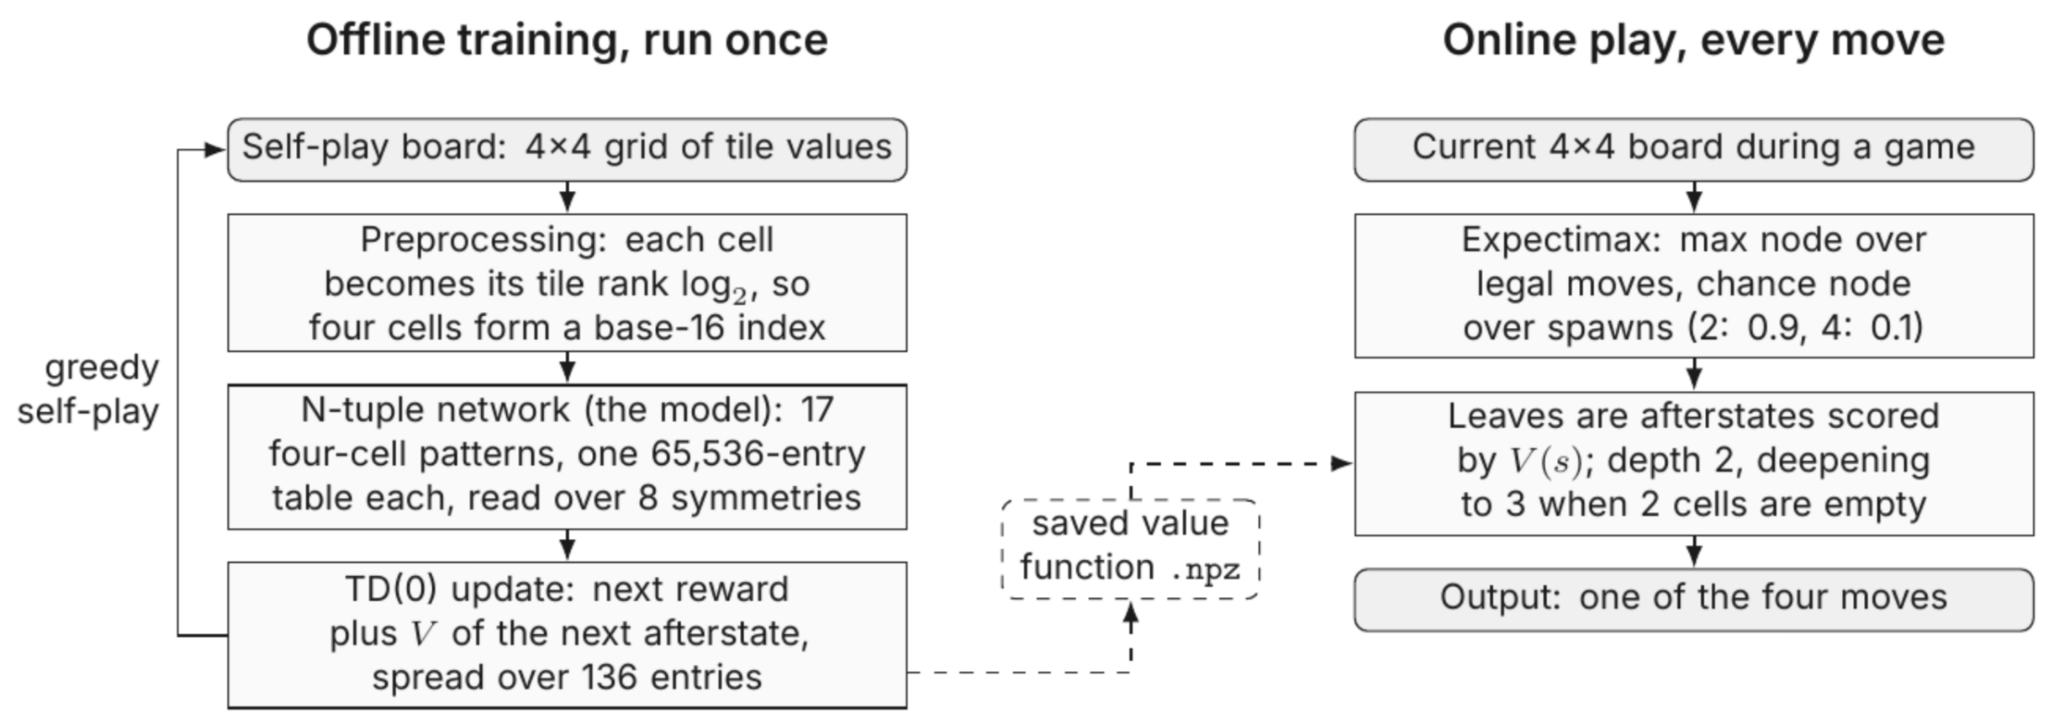
\includegraphics[width=0.80\textwidth]{image4.png}
\caption{The 2048 Master reinforcement learning pipeline.}
\end{figure}

\section*{Setting Up the 2048 Environment}

\subsection*{1. Board Representation}

We represent the 2048 board as a 4×4 NumPy array. Each cell stores the numerical value of the tile at that position, while an empty cell is represented by 0:

\begin{center}
\ttfamily
[0, 2, 0, 0]\quad [0, 0, 0, 0]\quad [0, 0, 4, 0]\quad [2, 0, 0, 0]
\end{center}

This representation allows the environment to perform board operations efficiently and provides the current game state directly to the AI agents.

\subsection*{2. Movement and Merging}

A single move consists of sliding all tiles toward the selected direction and merging adjacent tiles with the same value. For a left move, we remove empty cells, merge equal adjacent tiles, then slide the row again:

\begin{center}
\ttfamily Before: [2, 2, 4, 0]\quad Merge: [4, 0, 4, 0]\quad Slide: [4, 4, 0, 0]
\end{center}

Rather than implementing four independent movement algorithms, we reuse the same left-movement logic through board transformations:

\begin{itemize}
  \item Left: apply the left-movement logic directly.
  \item Right: reverse each row, apply left movement, then reverse it back.
  \item Up: transpose the board, apply left movement, then transpose it back.
  \item Down: transpose the board, apply right movement, then transpose it back.
\end{itemize}

This reduces duplicated code and keeps the merging behavior consistent across all directions.

\begin{figure}[H]
\centering
\codeshot[0.30\textwidth]{image13.png}
\caption{Code excerpt implementing left movement and merging.}
\end{figure}

\subsection*{3. Random Tile Spawning}

At the beginning of a game, two tiles are placed on randomly selected empty cells. After each legal move, the environment randomly selects an empty cell and places either a 2, with 90\% probability, or a 4, with 10\% probability. The movement functions return a \texttt{changed} flag, so a new tile is spawned only when the move modified the board. This makes 2048 a stochastic environment: the agent controls its actions, but it cannot control where or which value the next tile will appear.

\subsection*{4. Rewards}

The environment uses the score increase from tile merges as the immediate reward. When two equal tiles merge, the resulting tile's value is added to the score. For example, $[4,4]\rightarrow[8]$ gives a reward of 8. A move that only rearranges tiles receives a reward of 0. If multiple merges occur, their values are added to produce the total reward for that transition.

\section*{Building the N-Tuple Value Function}

The RL agent needs a value function $V(s)$ that estimates how good a board position is. We represent it with an N-tuple network, a set of lookup tables that evaluate a board by summing selected entries. An N-tuple network captures useful local board structure with compact tables that can be trained efficiently using TD learning.

\textbf{Tile ranks.} Every tile is a power of two, so instead of storing the value itself, we store its exponent. An empty cell becomes 0, and the tiles 2, 4 and 8 become 1, 2 and 3. This gives each cell one of 16 possible symbols.

\textbf{Tuple patterns.} A tuple is a fixed pattern of four cells. We use 17 tuples: the four rows, the four columns, and the nine overlapping 2×2 squares. These patterns capture the local interactions used to evaluate a board.

\begin{figure}[H]
\centering
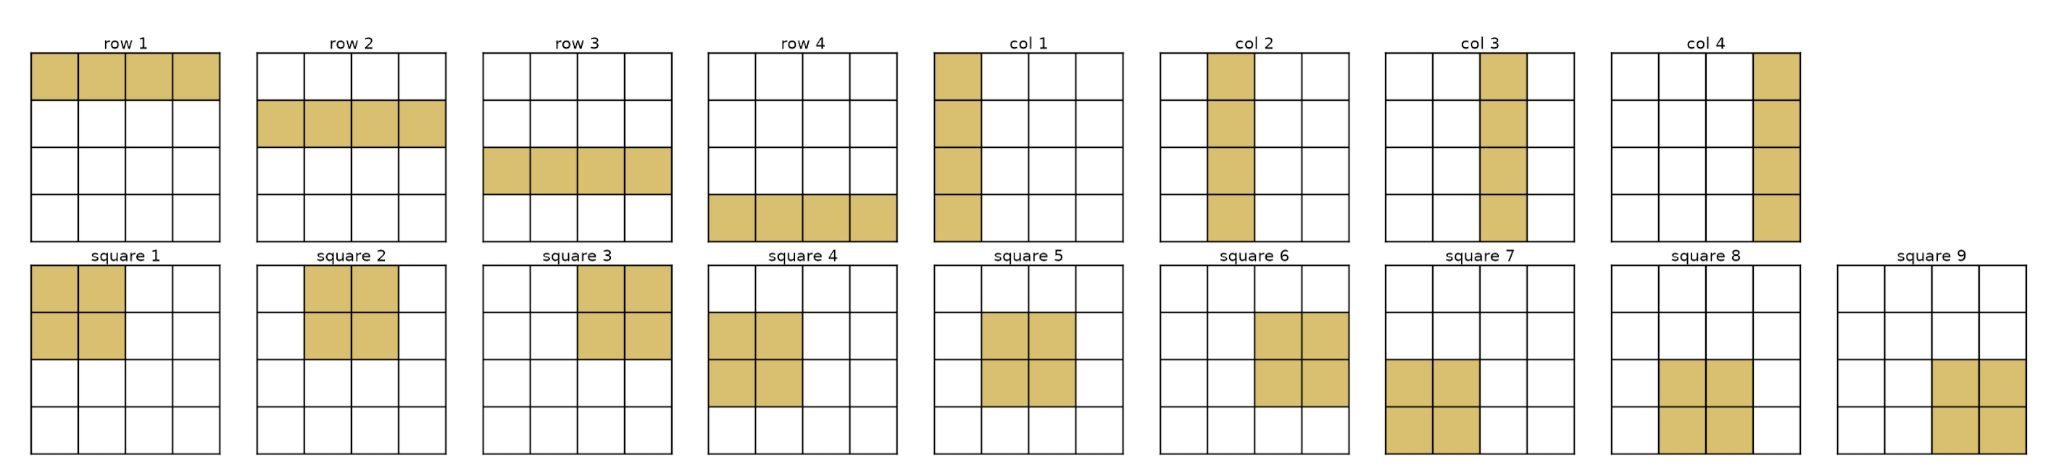
\includegraphics[width=0.86\textwidth]{image1.png}
\caption{The 17 four-cell tuple patterns.}
\end{figure}

\textbf{Lookup tables.} Each tuple pattern has its own lookup table, with one slot for every possible combination of values its four cells can contain. With 16 possible values per cell, each table contains $16^4=65{,}536$ slots. The network reads the slot selected by each pattern and sums the values it finds. Initially, all slots are zero.

\textbf{Base-16 encoding.} The four values in each tuple are converted into a single table index. The first cell contributes the units digit, while the remaining cells contribute multiples of 16, 256 and 4096. The tiles $[8,4,2,2]$ have exponents $[3,2,1,1]$, which encode as $3+2(16)+1(256)+1(4096)=4387$.

\begin{figure}[H]
\centering
\codeshot[0.58\textwidth]{image5.png}
\caption{Base-16 tuple encoding in the N-tuple network.}
\end{figure}

\textbf{Symmetry handling.} Rotated and reflected versions of the same board are strategically equivalent. Each board has eight orientations: four rotations and four rotations of a reflected version. We evaluate each board across all eight orientations using the same lookup tables. With 17 patterns and 8 orientations, each board contributes to 136 table entries. During training, the TD correction is divided evenly across these entries. We use \texttt{np.add.at} so entries selected more than once are updated correctly.

\begin{figure}[H]
\centering
\codeshot[0.42\textwidth]{image12.png}
\caption{Symmetry-aware evaluation and duplicate-safe updates.}
\end{figure}

\section*{Training with TD Learning}

We train the N-tuple value function through self-play. Its lookup tables are initially zero. As the agent plays games, TD updates adjust these values based on the rewards and future afterstates it encounters.

\subsection*{1. Afterstates}

An afterstate is the board immediately after the player's move has been applied, but before the random tile is spawned. A move in 2048 is deterministic, so afterstates represent the direct result of the agent's decision before randomness enters. This lets the agent evaluate the resulting board for each legal action directly.

\subsection*{2. TD Update}

For each possible action, the trainer evaluates the resulting afterstate by combining the immediate merge reward with the learned value of that afterstate. The action with the highest value is selected:

\begin{align*}
Q(s,a) &= r(s,a)+V(s'_a),\\
\text{target} &= r_{t+1}+V(s'_{t+1}),\\
\delta_t &= \text{target}-V(s'_t),\\
V(s'_t) &\leftarrow V(s'_t)+\alpha\delta_t.
\end{align*}

The value function estimates future rewards from an afterstate, so the immediate reward is handled separately during action selection. A terminal state has no future reward, so its TD target is zero.

\subsection*{3. Self-Play Training Loop}

The agent generates training data by repeatedly playing complete games of 2048. For each episode:

\begin{enumerate}
  \item Start a new board and spawn the initial two tiles.
  \item Test the four moves and discard actions that do not change the board.
  \item Apply each legal action without spawning a tile, then calculate its reward plus N-tuple value.
  \item Choose the action with the highest estimated value, execute it, and spawn a random tile.
  \item Calculate the TD target and error, then update the previous afterstate's N-tuple values.
  \item Continue until no legal moves remain, then start the next episode.
\end{enumerate}

\begin{figure}[H]
\centering
\codeshot[0.64\textwidth]{image11.png}
\caption{The main TD self-play update.}
\end{figure}

\subsection*{4. Training Configuration}

We trained the agent for 10,000 episodes to expose the value function to a wide range of board configurations. We experimented with different learning rates and selected the final value based on training performance and stability. Checkpoints are saved as \texttt{.npz} files containing the current N-tuple lookup tables, allowing training to resume without starting from zero.

\begin{figure}[H]
\centering
\codeshot[0.45\textwidth]{image6.png}
\caption{The training configuration excerpt.}
\end{figure}

\subsection*{5. Monitoring Training Progress}

We record each episode's score and calculate the average score. An increasing average indicates that the agent is generally learning to produce better game outcomes over time.

\begin{figure}[H]
\centering
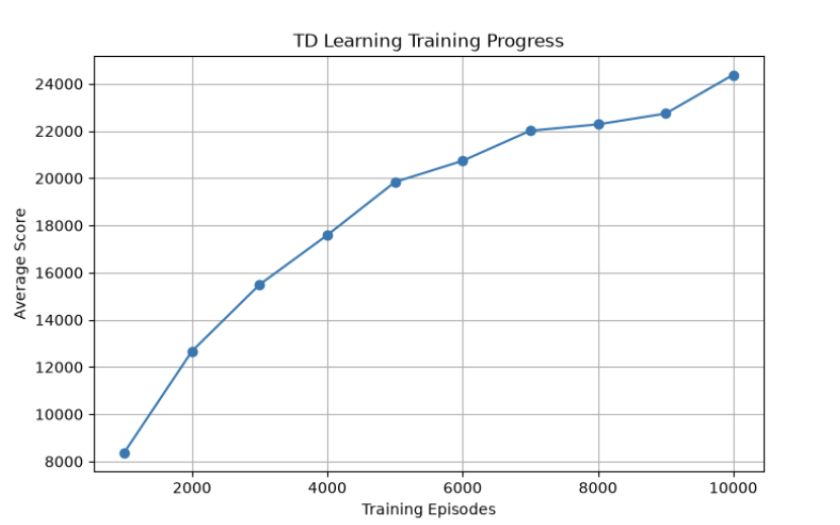
\includegraphics[width=0.40\textwidth]{image3.png}
\caption{Average score during 10,000 self-play episodes.}
\end{figure}

\section*{Integrating the Learned Value Function with Expectimax}

Expectimax needs a model of the game's randomness and a way to evaluate board positions. Chance nodes model the random spawning of a 2 or 4 tile. Our original Expectimax agent used a hand-designed heuristic. For the RL agent, we replaced that heuristic with the value function learned through TD self-play.

The search alternates between max nodes, where the agent chooses the best legal move, and chance nodes. We used a search depth of 2:

\begin{center}
max node $\rightarrow$ chance node $\rightarrow$ max node $\rightarrow$ chance node $\rightarrow$ evaluation function
\end{center}

At the leaf nodes, the N-tuple network evaluates the resulting board. Expectimax then determines which initial move has the highest expected outcome.

\begin{figure}[H]
\centering
\codeshot[0.55\textwidth]{image10.png}
\caption{The evaluation function used at Expectimax leaf nodes.}
\end{figure}

\section*{Evaluating the Agent}

We compared the Random agent, heuristic Expectimax, and Expectimax + RL in the same environment. The two Expectimax agents use the same depth-2 search; only their leaf evaluation differs. Each agent played 30 games.

\begin{table}[H]
\centering
\fontsize{7.5}{8.5}\selectfont
\setlength{\tabcolsep}{3.2pt}
\begin{tabular}{lrrrrrrr}
\toprule
\textbf{Agent} & \textbf{Games} & \textbf{Avg} & \textbf{Median} & \textbf{Best} & \textbf{Best tile} & \textbf{Reached 2048} & \textbf{ms/move} \\
\midrule
Random & 30 & 1,178 & 990 & 3,076 & 256 & 0/30 & 0.0 \\
Expectimax (heuristic) & 30 & 14,724 & 15,698 & 27,308 & 2,048 & 5/30 & 8.8 \\
Expectimax + RL & 30 & 62,244 & 66,646 & 120,744 & 8,192 & 30/30 & 12.9 \\
\bottomrule
\end{tabular}
\caption{Results from 30 games per agent.}
\end{table}

The RL agent achieved an average score more than four times higher than heuristic Expectimax and reached 2048 in all 30 games. Its best game reached 8192 with a score of 120,744. The RL agent takes about 4 ms more per move, which remains fast enough for real-time gameplay. Since both Expectimax agents use the same search, the difference comes from the learned N-tuple value function.

\section*{UI: The Pygame Interface}

The UI is separated from the game logic. The renderer displays the game, the environment handles the rules and state, and the AI agents independently select actions. The main menu offers the three agents and the comparison screen, selected with keys 1 to 4 or by clicking the buttons.

\begin{figure}[H]
\centering
\begin{minipage}[t]{0.31\textwidth}\centering
\codeshot[\linewidth]{image15.png}\\[-0.2em]
\footnotesize Main menu
\end{minipage}\hfill
\begin{minipage}[t]{0.31\textwidth}\centering
\codeshot[\linewidth]{image16.png}\\[-0.2em]
\footnotesize Agent gameplay
\end{minipage}\hfill
\begin{minipage}[t]{0.31\textwidth}\centering
\codeshot[\linewidth]{image14.png}\\[-0.2em]
\footnotesize Comparison screen
\end{minipage}
\caption{The Pygame interface.}
\end{figure}

Picking an agent starts a game and the agent plays by itself. Tiles slide and merge with animation, and the score updates in the header. Press \texttt{R} to restart, or \texttt{Esc} to return to the menu. When the game ends, an overlay shows the final score and best tile. The comparison screen runs five games per agent and reports the average score, best score and highest tile.

\section*{Troubleshooting}

\subsection*{Problem 1: \texttt{ModuleNotFoundError: No module named 'agents'}}

Running \texttt{python3 training/td\_learning.py} directly can fail because Python does not treat the project root as the package root. From the project root, run:

\begin{center}\texttt{python3 -m training.td\_learning}\end{center}

\subsection*{Problem 2: \texttt{ModuleNotFoundError: No module named 'pygame'}}

This means the current Python environment does not have the required dependencies. From the project root, run:

\begin{center}\texttt{pip install -r requirements.txt}\qquad\texttt{python3 main.py}\end{center}

\section*{Conclusion}

We built the environment, trained an N-tuple value function through TD self-play, and used it in Expectimax to replace the hand-designed heuristic.

{\footnotesize The authors retain full copyright of this guide and grant Simon Fraser University (SFU) permission to publish and share it for academic and educational purposes, including use by future students.}

\end{document}
